\documentclass[a4paper, 12pt]{article}
\usepackage{pgfplots}
\usepackage{mathtools}

%% Listings With Code-Styling and Grey Background
\usepackage{float}
\usepackage{listings} 
\usepackage{xcolor}
\usepackage{mdframed}
\usepackage{graphicx}
\definecolor{code-gray}{gray}{0.93}

%% Custom FSM's
\usepackage{tikz}
\usetikzlibrary{automata, positioning, arrows}
\tikzset{very thick, ->, >=stealth', node distance=6cm, every state/.style={thick, fill=gray!10}, initial text=$ $}

%% Automatic Word Formatting
\usepackage{xspace}
\newcommand*{\Vivado}{\textit{Vivado}\xspace} % Italicize Vivado
\newcommand*{\SV}{\textbf{SystemVerilog}\xspace} % Bold SystemVerilog

%% Clickable links in the output PDF
\usepackage{hyperref}
\hypersetup{colorlinks=true, linktoc=all, linkcolor=black}

%% Figure Numbering Within Sections
\let\counterwithout\relax
\let\counterwithin\relax
\usepackage{chngcntr}
\counterwithin{figure}{section}

%% Macros for logic timing diagrams
\newcounter{wavenum}
\setlength{\unitlength}{1cm}
% advance clock one cycle, not to be called directly
\newcommand*{\clki}{
  \draw (t_cur) -- ++(0,.3) -- ++(.5,0) -- ++(0,-.6) -- ++(.5,0) -- ++(0,.3)
    node[time] (t_cur) {};
}
\newcommand*{\bitvector}[3]{
  \draw[fill=#3] (t_cur) -- ++( .1, .3) -- ++(#2-.2,0) -- ++(.1, -.3)
                         -- ++(-.1,-.3) -- ++(.2-#2,0) -- cycle;
  \path (t_cur) -- node[anchor=mid] {#1} ++(#2,0) node[time] (t_cur) {};
}
% \known{val}{length}
\newcommand*{\known}[2]{
    \bitvector{#1}{#2}{white}
}
% \unknown{length}
\newcommand*{\unknown}[2][XXX]{
    \bitvector{#1}{#2}{black!20}
}
% \bit{1 or 0}{length}
\newcommand*{\bit}[2]{
  \draw (t_cur) -- ++(0,.6*#1-.3) -- ++(#2,0) -- ++(0,.3-.6*#1)
    node[time] (t_cur) {};
}
% \unknownbit{length}
\newcommand*{\unknownbit}[1]{
  \draw[ultra thick,black!50] (t_cur) -- ++(#1,0) node[time] (t_cur) {};
}
% \nextwave{name}
\newcommand{\nextwave}[1]{
  \path (0,\value{wavenum}) node[left] {#1} node[time] (t_cur) {};
  \addtocounter{wavenum}{-1}
}
% \clk{name}{period}
\newcommand{\clk}[2]{
    \nextwave{#1}
    \FPeval{\res}{(\wavewidth+1)/#2}
    \FPeval{\reshalf}{#2/2}
    \foreach \t in {1,2,...,\res}{
        \bit{\reshalf}{1}
        \bit{\reshalf}{0}
    }
}

% \begin{wave}[clkname]{num_waves}{clock_cycles}
\newenvironment{wave}[3][clk]{
  \begin{tikzpicture}[draw=black, yscale=.7,xscale=1]
    \tikzstyle{time}=[coordinate]
    \setlength{\unitlength}{1cm}
    \def\wavewidth{#3}
    \setcounter{wavenum}{0}
    \nextwave{#1}
    \foreach \t in {0,1,...,\wavewidth}{
      \draw[dotted] (t_cur) +(0,.5) node[above] {t=\t} -- ++(0,.4-#2);
      \clki
    }
}{\end{tikzpicture}}

%$ Specific Line Breaks
% See https://tex.stackexchange.com/questions/26174/ for details
\usepackage[british]{babel} 

%% Page Margins
\usepackage[margin=1.00in]{geometry}

% Beginning of Document
\begin{document}
\counterwithin{lstlisting}{section} % Listings are numbered within sections
% Title
\title{ECE 440 - Homework \#3}
\author{Collin Heist}
\date{\today}
\maketitle

% Table of Content and Listings
\pagenumbering{arabic}

% Beginning of Report
\section{Exercise 3.1}
\subsection{RegWithBenefits Module}
\begin{mdframed}[backgroundcolor=code-gray, roundcorner=10pt, innerleftmargin=15, innertopmargin=5, innerbottommargin=5]	
\lstinputlisting[breaklines, language=Verilog, caption=Register 'With Benefits' Module, tabsize=2, label={lst:fsm-module}]{regWithBenefits.sv}
\end{mdframed}

\subsection{Testbench}
\begin{mdframed}[backgroundcolor=code-gray, roundcorner=10pt, innerleftmargin=15, innertopmargin=5, innerbottommargin=5]	
\lstinputlisting[breaklines, language=Verilog, caption=8-bit Register Testbench, tabsize=2, label={lst:fsm-module}]{testbench.sv}
\end{mdframed}

\subsection{Simulation Results}
Although it might be hard to see, the behavioral simulation results are exactly as expected. The asynchronous reset going low (as it is an active low signal) immediately results in \textbf{reg\_out} becoming all zeros, and the shifting operation works as expected.

\begin{figure}[H]
\centering
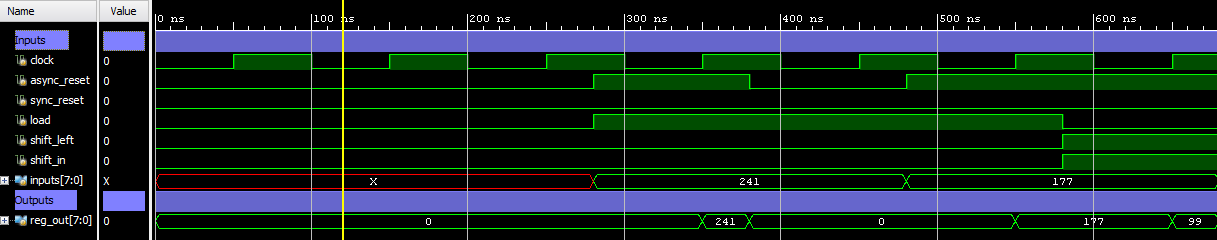
\includegraphics[width=\textwidth]{Sources/Behav-Sim.PNG}
\caption{Results of the Behavioral Simulation.}
\end{figure}

The TCL console print statements show the shifting in and shifting left operations working as expected.

\begin{figure}[H]
\centering
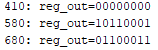
\includegraphics[width=0.6\textwidth]{Sources/console.PNG}
\caption{Results of the Behavioral Simulation.}
\end{figure}

\end{document}